\documentclass[tikz,border=0pt]{standalone}
% Shared style for docs/*.tex diagrams: Horizon dark palette (as analysis/style.mplstyle).
\usepackage[scaled]{helvet}
\renewcommand\familydefault{\sfdefault}
\usetikzlibrary{arrows.meta,backgrounds,fit,calc,shapes.geometric}
\pgfdeclarelayer{ns}
\pgfsetlayers{background,ns,main}

\definecolor{bg}{HTML}{1C1E26}
\definecolor{fg}{HTML}{FFFFFF}
\definecolor{pink}{HTML}{E95378}
\definecolor{teal}{HTML}{25B0BC}
\definecolor{peach}{HTML}{FAB795}
\definecolor{purple}{HTML}{B877DB}
\definecolor{green}{HTML}{27D797}
\definecolor{muted}{HTML}{9DA0C2}

\tikzset{
  every node/.style={font=\small, text=fg},
  diagram/.style={background rectangle/.style={fill=bg}, show background rectangle, inner frame sep=14pt},
  box/.style={draw, rounded corners=3pt, line width=0.9pt, align=center,
              minimum height=0.9cm, minimum width=2.2cm, inner sep=4pt},
  ros/.style={box, draw=purple, fill=purple!22!bg},
  radio/.style={box, draw=teal, fill=teal!22!bg},
  mine/.style={box, draw=pink, fill=pink!22!bg},
  ns/.style={draw=muted, dashed, rounded corners=6pt, line width=0.7pt, inner sep=12pt},
  nslabel/.style={font=\footnotesize\itshape, text=muted, anchor=north west},
  data/.style={-{Latex[length=2.4mm]}, line width=1pt, draw=peach},
  back/.style={-{Latex[length=2.4mm]}, line width=1pt, draw=green},
  lbl/.style={font=\scriptsize, text=muted, fill=bg, inner sep=1.5pt},
}

\begin{document}
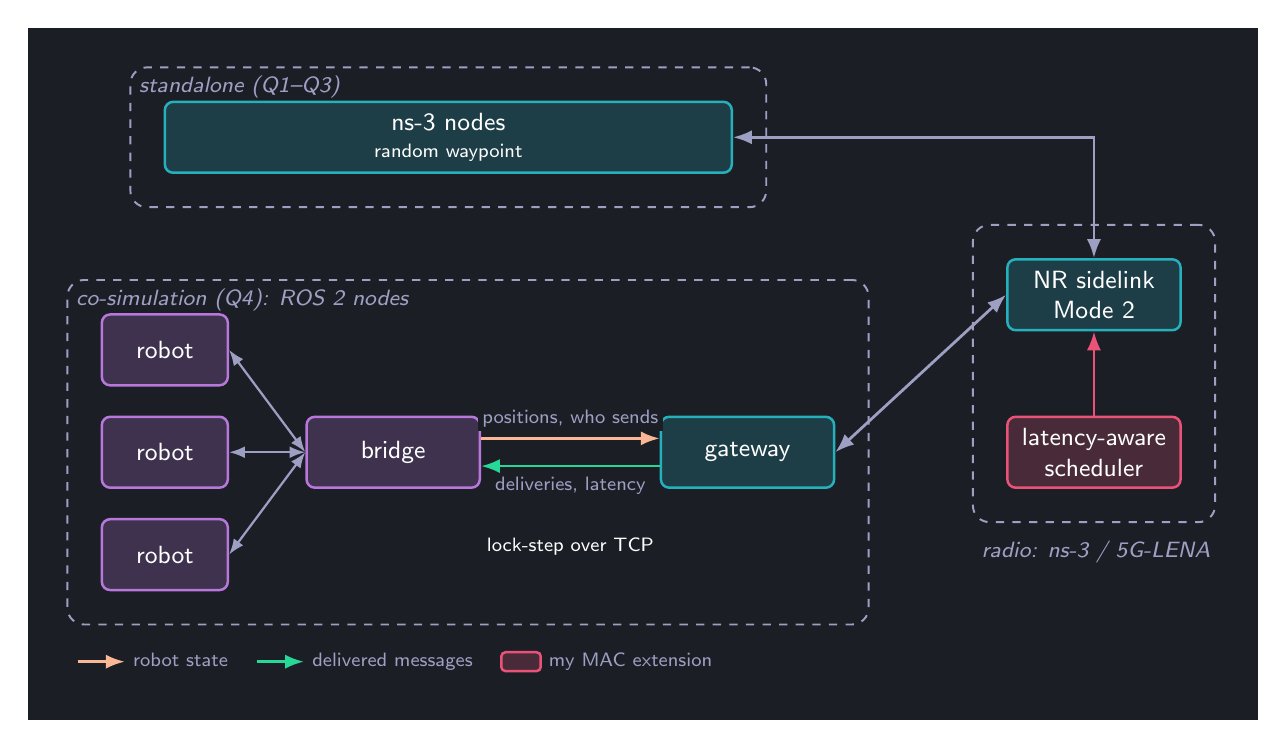
\begin{tikzpicture}[diagram, rbt/.style={ros, minimum width=1.6cm}]
  \node[radio, minimum width=7.2cm] (bi) at (3.6, 2.3)
  {ns-3 nodes\\[-1pt]{\scriptsize random waypoint}};

  \node[rbt] (r1) at (0,-0.4) {robot};
  \node[rbt] (r2) at (0,-1.7) {robot};
  \node[rbt] (rn) at (0,-3.0) {robot};
  \node[ros] (br) at (2.9,-1.7) {bridge};
  \node[radio] (gw) at (7.4,-1.7) {gateway};

  \node[radio] (sl)  at (11.8, 0.3)  {NR sidelink\\Mode 2};
  \node[mine]  (sch) at (11.8,-1.7)  {latency-aware\\scheduler};

  \foreach \r in {r1,r2,rn} { \draw[<->, -{Latex[length=2mm]}, {Latex[length=2mm]}-{Latex[length=2mm]}, line width=0.8pt, draw=muted] (\r.east) -- (br.west); }
  \draw[data] ([yshift=5pt]br.east) -- node[lbl, above=2pt] {positions, who sends} ([yshift=5pt]gw.west);
  \draw[back] ([yshift=-5pt]gw.west) -- node[lbl, below=2pt] {deliveries, latency} ([yshift=-5pt]br.east);
  \node[lbl, text=fg, align=center] at ($(br.east)!0.5!(gw.west)+(0,-1.2)$) {lock-step over TCP};

  \draw[{Latex[length=2.4mm]}-{Latex[length=2.4mm]}, line width=1pt, draw=muted] (bi.east) -| (sl.north);
  \draw[{Latex[length=2.4mm]}-{Latex[length=2.4mm]}, line width=1pt, draw=muted] (gw.east) -- (sl.west);
  \draw[draw=pink, line width=1pt, -{Latex[length=2.4mm]}] (sch) -- (sl);

  \begin{pgfonlayer}{ns}
    \node[ns, fit=(bi)] (nsA) {};
    \node[nslabel] at (nsA.north west) {standalone (Q1--Q3)};
    \node[ns, fit=(r1)(rn)(br)(gw)] (nsB) {};
    \node[nslabel] at (nsB.north west) {co-simulation (Q4): ROS 2 nodes};
    \node[ns, fit=(sl)(sch)] (nsR) {};
    \node[nslabel, anchor=north west] at ($(nsR.south west)+(0,-0.1)$) {radio: ns-3 / 5G-LENA};
  \end{pgfonlayer}

  \node[anchor=north west, font=\scriptsize, text=muted] at ($(nsB.south west)+(0,-0.2)$) {
    \tikz[baseline=-0.6ex]\draw[data] (0,0) -- (0.6,0); robot state \quad
    \tikz[baseline=-0.6ex]\draw[back] (0,0) -- (0.6,0); delivered messages \quad
  \tikz[baseline=-0.6ex]\draw[draw=pink, fill=pink!22!bg, line width=0.9pt, rounded corners=1.5pt] (0,-0.12) rectangle (0.5,0.12); my MAC extension};
\end{tikzpicture}
\end{document}
